\section{Resultados del Algoritmo Genético}

En esta sección presentamos los resultados obtenidos con el AG. Para obtener la matriz con la asignación final se simularon $6$ generaciones (población inicial más 5 reemplazamientos). El tamaño de la población para cada generación es $10$. El número de genes varía dependiendo de cada asignación.


En la \figurename{~\ref{EjcalifMejoresHijos}} vemos las calificaciones de la mejor asignación por generación. Observamos que la mejora en la calificación es considerable de la población inicial a la segunda generación. Notamos que la calificación del mejor elemento de la generación 5 fue menor al de la generación 4.

\begin{figure}[H]
\centering
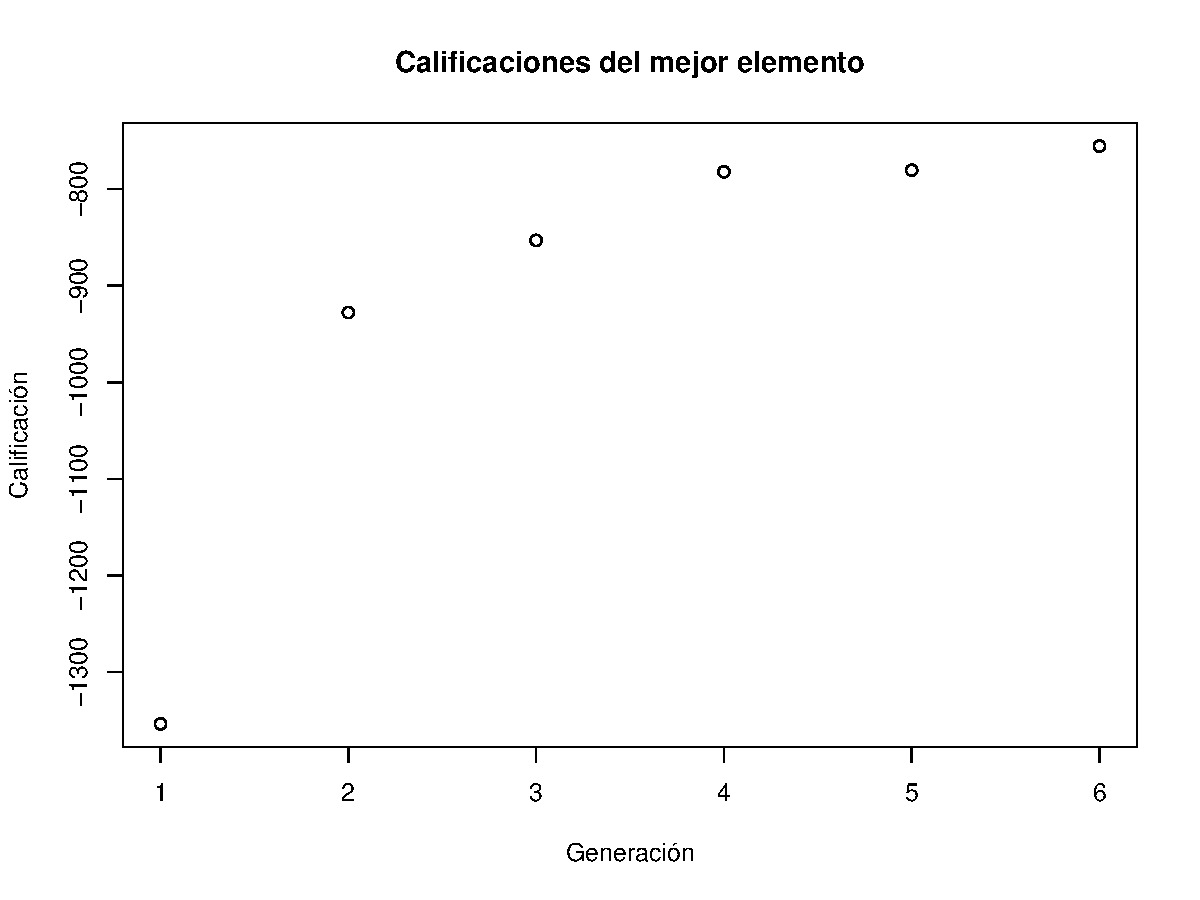
\includegraphics[width=\textwidth]{calif_mejores_hijos.pdf} %scale = 0.7
\caption[\textit{Calificaciones de mejores asignaciones}]{\textit{Se muestran las calificaciones de la mejor asignación por generación. Se observa una mejora considerable en la calificación de la generación 1 a la 2.}}\label{EjcalifMejoresHijos}
\end{figure}

%En la \figurename{~\ref{EjcalifAsig}} vemos las calificaciones de las asignaciones.
%
%\begin{figure}[H]
%\centering
%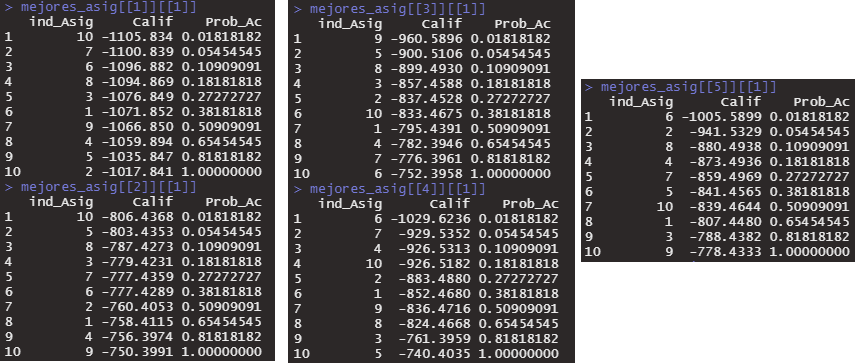
\includegraphics[width=\textwidth]{ej_calif_asignaciones} %scale = 0.7
%\caption{\textit{Ejemplo con calificaciones de asignaciones.}}\label{EjcalifAsig}
%\end{figure}

En la \figurename{~\ref{EjcalifAsig_x_generacion}} vemos las calificaciones de las asignaciones por generación. Cada línea representa una generación. De abajo hacia arriba se tiene de la primer población a la sexta. Podemos ver que las calificaciones de las poblaciones 4 y 5 son muy parecidas. Al igual que en la \figurename{~\ref{EjcalifMejoresHijos}}, se puede observar una mejora considerable en las calificaciones de las asignaciones de la generación 1 a la 2.

\begin{figure}[H]
\centering
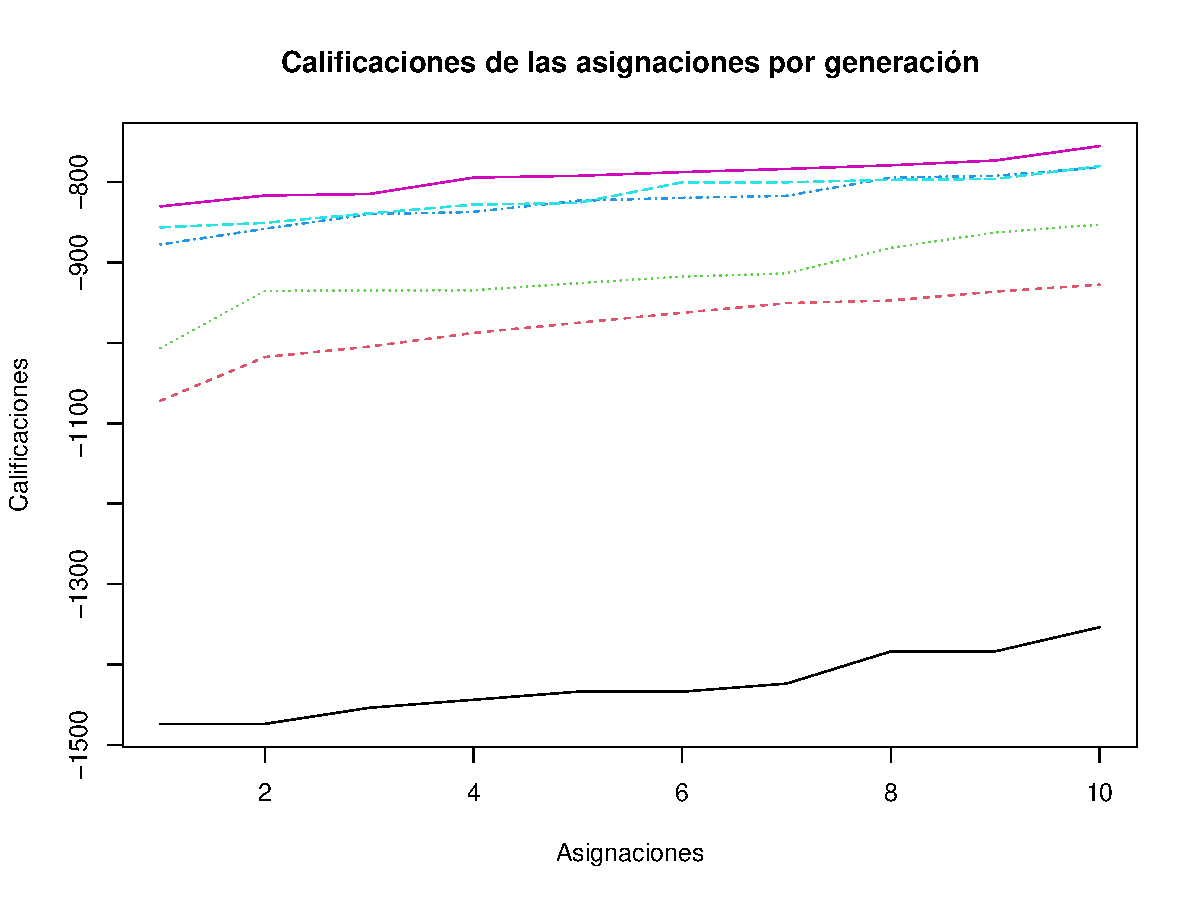
\includegraphics[width=\textwidth]{calif_asig_x_generacion.pdf} %scale = 0.7
\caption[\textit{Calificaciones de asignaciones por generación}]{\textit{Se muestran las calificaciones de las asignaciones por generación. Se observa una mejora considerable en la calificación de la generación 1 a la 2.}}\label{EjcalifAsig_x_generacion}
\end{figure}


Sabemos que la asignación final es el mejor elemento de la última generación. En la \tablename{~\ref{submatAsigFinal}} presentamos una submatriz de la asignación final. Cabe aclarar que los datos se ordenaron con respecto a la materia (en orden alfabético) y por hora (de menor a mayor). La matriz completa se puede ver el el Apéndice \ref{Ej_AsigFinal}.

\begin{table}[H]
\centering
\begin{tabular}{|c|p{7cm}|p{4.7cm}|c|}
\hline
\textbf{ } & \textbf{Materia} & \textbf{Profesor} & \textbf{Horario} \\ \hline
1 & Administración Actuarial del Riesgo & Ricardo Villegas Azcorra & 7 \\ \hline
108 & Análisis Numérico & Ursula Xiomara Iturrarán Viveros & 10 \\ \hline
109 & Análisis Numérico & Úrsula Xiomara Iturrarán Viveros & 10 \\ \hline
118 & Cálculo Diferencial e Integral I & Javier Fernández García & 7 \\ \hline
153 & Cálculo Diferencial e Integral III & Javier Fernández García & 11 \\ \hline
161 & Cálculo Diferencial e Integral IV & Héctor Méndez Lango & 10 \\ \hline
442 & Modelos de Supervivencia y de Series de Tiempo & Margarita Elvira Chávez Cano & 10 \\ \hline
444 & Modelos de Supervivencia y de Series de Tiempo & Rubén Ugalde Franco & 17 \\ \hline
445 & Modelos no Paramétricos y de Regresión & Margarita Elvira Chávez Cano & 9 \\ \hline
448 & Modelos no Paramétricos y de Regresión & Lizbeth Naranjo Albarrán & 11 \\ \hline
449 & Modelos no Paramétricos y de Regresión & Jaime Vázquez Alamilla & 12 \\ \hline
470 & Probabilidad I & Jaime Vázquez Alamilla & 8 \\ \hline
476 & Probabilidad I & Bibiana Obregón Quintana & 14 \\ \hline
496 & Procesos Estocásticos I & Sergio Iván López Ortega & 15 \\ \hline
603 & Variable Compleja I & Carisa Cano Figueroa & 13 \\ \hline
\end{tabular}
\caption[\textit{Submatriz con asignación final}]{\textit{Se muestra una submatriz de la asignación final. Cada renglón tiene la información de un grupo con una materia, profesor y horario asignado.}}\label{submatAsigFinal}
\end{table}